% Compile from this directory: pdflatex main.tex
% Regenerate figures: python ../scripts/build_report_figures.py
\documentclass[11pt,a4paper]{article}
\usepackage[margin=2.2cm]{geometry}
\usepackage{graphicx}
\usepackage{booktabs}
\usepackage{amsmath}
\usepackage{microtype}
\usepackage[hidelinks]{hyperref}
\usepackage{tikz}
\usetikzlibrary{arrows.meta,positioning}

\title{\textbf{Predicting aqueous diffusion coefficients}\\{\large from SMILES and temperature (Han et al.\ SI)}}
\author{Project summary}
\date{\today}

\begin{document}
\maketitle

\begin{abstract}
We built an end-to-end pipeline from the supplemental Excel file \texttt{jp5c01881\_si\_002.xlsx} (Table~S2) to neural regressors that predict $\log_{10} D$ for water, conditioned on molecular structure and temperature. Models are evaluated on \emph{molecule-level} held-out test sets: a random split and a harder scaffold split. A graph neural network (GNN) slightly outperforms a Morgan-fingerprint MLP; both dominate trivial and linear baselines.
\end{abstract}

\section*{Why this setup}
Diffusion coefficients $D$ span many orders of magnitude. Training on $D$ directly would overweight large values, so we predict $\log_{10}(D)$ with Huber loss and report errors in log space and on back-transformed $D$. Temperature stays in kelvin but is normalized using \textbf{training-set} statistics only. Splits are by \textbf{canonical SMILES}, never by row: otherwise the same compound at different $T$ would leak between train and test. A \textbf{scaffold} split asks for generalization to chemotypes not seen in training---often stricter than random-by-molecule splits.

\section*{What we implemented}
Figure~\ref{fig:pipe} sketches the flow. After RDKit canonicalization and deduplication of $(\text{SMILES},T)$ (mean $D$), we featurize with either Morgan fingerprints or a PyTorch~Geometric molecular graph, fuse with scaled $T$, and train with early stopping on validation loss. Checkpoints and metrics live under \texttt{artifacts/}; figures for this note are produced by \texttt{scripts/build\_report\_figures.py}.

\begin{figure}[ht]
  \centering
  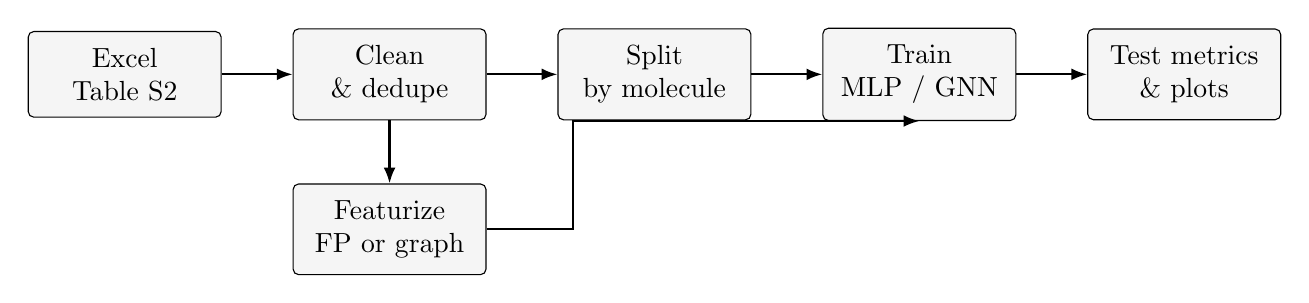
\begin{tikzpicture}[
    node distance=8mm and 9mm,
    box/.style={draw, rounded corners=2pt, align=center, inner sep=6pt, minimum width=2.45cm, fill=black!4},
    arr/.style={-{Latex[length=2mm]}, thick},
  ]
    \node[box] (x) {Excel\\Table S2};
    \node[box, right=of x] (c) {Clean\\\& dedupe};
    \node[box, right=of c] (s) {Split\\by molecule};
    \node[box, right=of s] (t) {Train\\MLP / GNN};
    \node[box, right=of t] (e) {Test metrics\\\& plots};
    \node[box, below=of c] (f) {Featurize\\FP or graph};
    \draw[arr] (x) -- (c);
    \draw[arr] (c) -- (s);
    \draw[arr] (s) -- (t);
    \draw[arr] (t) -- (e);
    \draw[arr] (c) -- (f);
    \draw[arr] (f.east) -- ++(1.1,0) |- (t.south);
  \end{tikzpicture}
  \caption{End-to-end pipeline: cleaning and splits use SMILES identity; models consume structure~+~scaled temperature.}
  \label{fig:pipe}
\end{figure}

\section*{Data snapshot (after cleaning)}
\begin{center}
\begin{tabular}{@{}lr@{}}
\toprule
Metric & Value \\
\midrule
Rows after dedupe & 20\,576 \\
Unique SMILES & 6\,909 \\
$T$ range (K) & 273.8 -- 394.0 \\
Duplicate pairs collapsed & 152 (mean $D$) \\
\bottomrule
\end{tabular}
\end{center}

\section*{How good are the models?}
Figure~\ref{fig:cmp} compares test RMSE and $R^2$ in $\log_{10} D$ for ridge (linear on FP$+T$), MLP, and GNN. The dashed line marks a constant \emph{mean}-$\log D$ baseline (RMSE $\approx 0.47$): learned models sit far below it. Figure~\ref{fig:med} shows median absolute relative error on linear $D$ on the test set (roughly ``typical fractional error'').

\begin{figure}[ht]
  \centering
  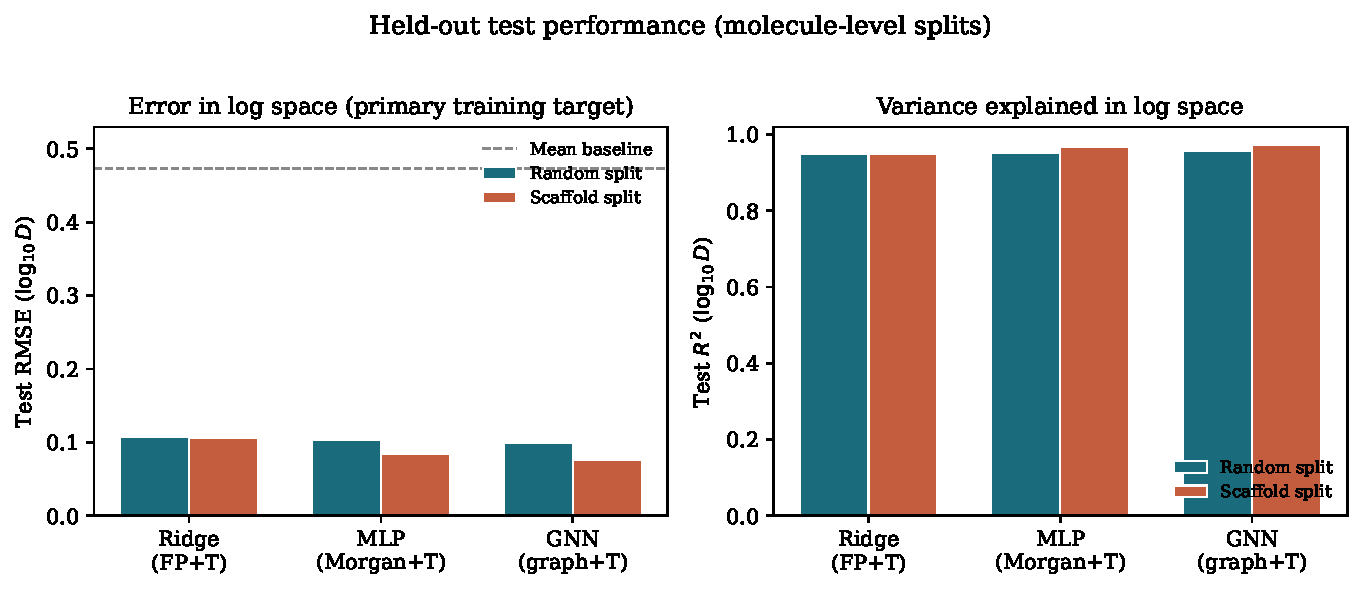
\includegraphics[width=\linewidth]{figures/model_comparison.pdf}
  \caption{Held-out \textbf{test} metrics for two molecule-level schemes: random vs scaffold. Lower RMSE / higher $R^2$ is better.}
  \label{fig:cmp}
\end{figure}

\begin{figure}[ht]
  \centering
  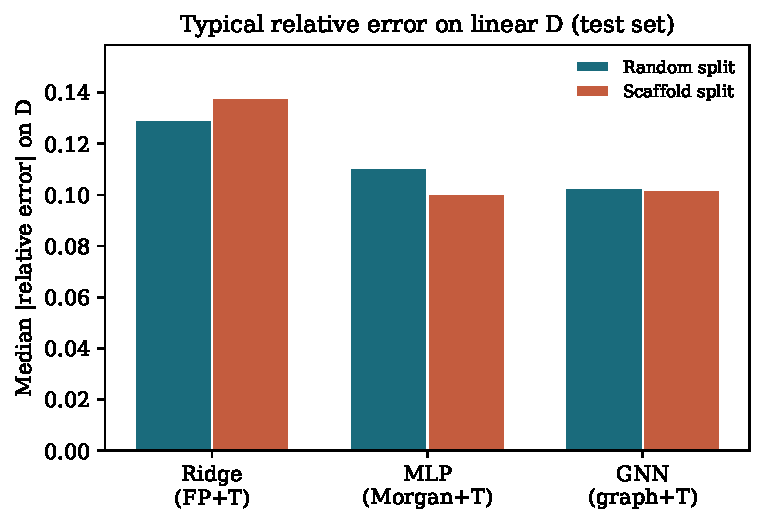
\includegraphics[width=0.72\linewidth]{figures/median_rel_error_D.pdf}
  \caption{Median $|\hat D - D|/D$ on the test set (robust to heavy-tailed $D$). Mean/median baselines are $\sim$0.77--0.79 (not shown).}
  \label{fig:med}
\end{figure}

\begin{table}[ht]
  \centering
  \caption{Representative test numbers (scaffold split; best-performing setup in our run).}
  \begin{tabular}{@{}lccc@{}}
    \toprule
    Model & RMSE $\log_{10}D$ & $R^2$ $\log_{10}D$ & Med.\ rel.\ err.\ on $D$ \\
    \midrule
    Ridge (FP$+T$) & 0.106 & 0.949 & 0.138 \\
    MLP & 0.084 & 0.968 & 0.101 \\
    GNN & \textbf{0.077} & \textbf{0.974} & \textbf{0.102} \\
    \bottomrule
  \end{tabular}
\end{table}

\section*{Scope and caveats}
The model is trained for \textbf{aqueous} diffusion only. Confirm $D$ \textbf{units} against the original paper when quoting absolute values. Predictions outside the observed $T$ range are extrapolation; the Python API can flag this using training $T$ bounds stored in checkpoints.

\end{document}
